\documentclass[12pt]{article}

\usepackage{fontawesome}
\usepackage{hyperref}
\usepackage{xurl}
\usepackage{graphicx}
\usepackage{float}
\usepackage{fancyvrb}
\usepackage[tagged, highstructure]{accessibility}
\usepackage{bookmark}
\usepackage{enumitem}

\hypersetup{
    colorlinks=false,
    pdfborder={0 0 0},
    pdftitle={Digital Forensics},
    pdfauthor={Adrianna Holden-Gouveia},
    pdfsubject={Information Security - Lab Assignment},
    pdflang={en-US},
    pdfkeywords={digital forensics, hashing, SHA-256, forensic copy, metadata, incident response}
}

% Configure PDF bookmarks for navigation
\bookmarksetup{
    numbered,
    open,
}

% Configure list spacing for better accessibility
\setlist{nosep}



\title{Digital Forensics}
\author{
        Adrianna Holden-Gouveia \\
        Website: \href{https://aholdengouveia.name}{aholdengouveia.name}\\ 
        \date{\vspace{-5ex}}
        %Email: \href{mailto:admin@aholdengouveia.name}{admin@aholdengouveia.name} \\
%        \faLinkedin{: aholdengouveia} \\
        \faGithub {: aholdengouveia} \\
        \faTwitter {: aholdengouveia} \\
        }

%S\date{\today}


\begin{document}

\maketitle

\section*{Accessibility Notice}
This document is also available in HTML format at:

Link: \href{https://aholdengouveia.name/InfoSec/labs/forensics.html}{\textbf{\nolinkurl{https://aholdengouveia.name/InfoSec/labs/forensics.html}}}

The HTML version provides enhanced accessibility features including keyboard navigation, screen reader support, responsive design, dark mode support, and high contrast options.

\section*{Learning Outcomes}
By the end of this lab, you will be able to:
\begin{itemize}
    \item Use hashes to show whether a file is an exact copy, or has been changed
    \item Make a forensic copy of a practice disk image, and prove it matches the original
    \item Identify the hidden evidence stored in a photo, and remove it before sharing
    \item Describe how an organization investigates and responds to an incident, using a real post-mortem
\end{itemize}

\section*{Lab Instructions}
Forensic investigators have to prove that the evidence they show in court is exactly what they collected. In this lab, you'll use hashes to prove files match, make a forensic copy, find hidden evidence in a photo, and read how a real company investigated an attack.

\textbf{Parts 1 and 2 use the terminal in your Kali or Mint virtual machine from Lab 1.} If you're new to the terminal, my Linux FAQ playlist, linked under Resources, shows how to open one and run commands. A few tips:
\begin{itemize}
    \item Type each command exactly, then press Enter. Spaces and capital letters matter.
    \item Copy and paste may not work between your computer and the virtual machine, so be ready to type the commands.
    \item Press the Up arrow to bring back the last command, so you can change it and run it again.
\end{itemize}
Part 3 uses a photo on your phone, and Part 4 is reading and writing.

\subsection*{Screenshots}
This lab asks for about 9 screenshots. Each screenshot should have your name, term, and year.  One of the easiest ways to do that is make a text document with your name and term/year on your computer and save it to use all term. Any screenshots that don't include this information won't be counted.

\begin{figure}[H]
    \centerline{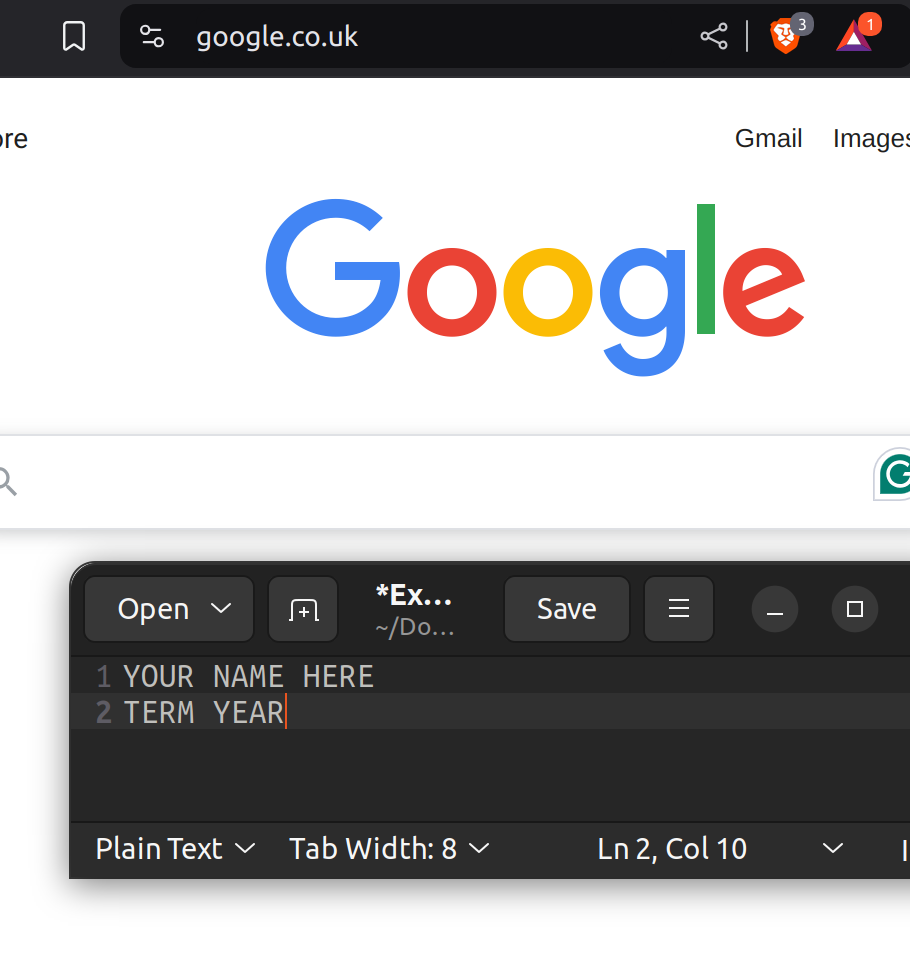
\includegraphics[scale=.2]{ExampleScreenshot.png}}
    \caption{This is an image of what each of your screenshots should look like}
    \alt{Example screenshot: a web browser showing the Google home page, with a small text editor window in front of it that says YOUR NAME HERE and TERM YEAR}
\end{figure}

\subsection*{Part 1: Hashing}
A hash is like a fingerprint for a file. If even one letter in the file changes, the hash changes completely. Investigators use SHA-256 hashes to prove a copy matches the original. In Linux, the command is \texttt{sha256sum}, followed by the file's name.

In your virtual machine, open the browser, and download my 2 practice evidence files, \texttt{evidence-a.txt} and \texttt{evidence-b.txt}, linked under Resources. They'll save to your Downloads folder. Then open a terminal, and go to that folder:
\begin{Verbatim}
cd Downloads
\end{Verbatim}
\begin{enumerate}
    \item Make a practice file, and hash it. Put your own name in place of Your Name. Take a screenshot.
\begin{Verbatim}
echo "Your Name is learning forensics" > myfile.txt
sha256sum myfile.txt
\end{Verbatim}
    \item Press the Up arrow to bring back the \texttt{echo} command, change one letter in the sentence, and run it again. Then hash the file again. Take a screenshot. How much of the hash changed?
    \item One of my evidence files is the original, and one has been tampered with. The SHA-256 hash of the original is:
\begin{Verbatim}
771da36bd7fd679da3116135250a1f4a84f03bdb49b972522ad8a596e73b8216
\end{Verbatim}
    Hash both files, and take a screenshot. Which one is the original?
\begin{Verbatim}
sha256sum evidence-a.txt evidence-b.txt
\end{Verbatim}
    \item Show what's inside both files, and take a screenshot. What was changed in the tampered file?
\begin{Verbatim}
cat evidence-a.txt evidence-b.txt
\end{Verbatim}
    \item Why does it matter that an investigator can prove a piece of evidence hasn't been changed? Use the tampered file as an example.
\end{enumerate}

\subsection*{Part 2: Make a Forensic Copy}
Investigators never work on the original drive. They make an exact copy, called a forensic image, prove it matches with a hash, and only work on the copy. You'll do the same with a small practice ``drive'' that you make yourself.

\textbf{Only run these commands in your virtual machine, and type them exactly.} The \texttt{dd} command copies raw data. If it's pointed at the wrong place, it can erase a real drive.

In the terminal, run these commands one at a time. Here's what each one does:
\begin{itemize}
    \item \texttt{cd} with nothing after it goes back to your home folder, and \texttt{mkdir forensics} makes a new folder called forensics. \texttt{cd forensics} goes into it.
    \item The first \texttt{dd} command makes a 10 MB practice drive, called \texttt{evidence.img}, filled with random data.
    \item \texttt{chmod 444} makes the practice drive read-only, so nothing can change it.
    \item The second \texttt{dd} command makes a forensic copy, called \texttt{copy.img}.
    \item \texttt{sha256sum} hashes both, so you can compare them.
\end{itemize}
\begin{Verbatim}
cd
mkdir forensics
cd forensics
dd if=/dev/urandom of=evidence.img bs=1M count=10
chmod 444 evidence.img
dd if=evidence.img of=copy.img bs=1M
sha256sum evidence.img copy.img
\end{Verbatim}
\begin{enumerate}[start=6]
    \item Take a screenshot showing both hashes. Do they match?
    \item Now change the copy. This command writes the letter X into the middle of the copy, which changes just 1 byte out of about 10 million. Then hash both again, and take a screenshot.
\begin{Verbatim}
printf 'X' | dd of=copy.img bs=1 seek=5000 conv=notrunc
sha256sum evidence.img copy.img
\end{Verbatim}
    \item Explain what happened to the hashes, and why. What would this mean if it happened to real evidence?
    \item In real investigations, a write blocker stops the computer from changing the original drive. Which command in this lab did something similar, and why does it matter?
\end{enumerate}

\subsection*{Part 3: Hidden Evidence in a Photo}
Photos you take often have hidden details saved inside them, called metadata or EXIF data. This can include the device, the date and time, and the exact location. This part uses your phone, not the virtual machine. Pick a photo you took with your phone, and look at its details:
\begin{itemize}
    \item \textbf{iPhone:} open the photo in Photos, and swipe up, or select the information button.
    \item \textbf{Android (Google Photos):} open the photo, and swipe up, or select the menu.
    \item \textbf{Windows:} right-click the photo, select Properties, then the Details tab.
    \item \textbf{Mac:} open the photo in Preview, select Tools, then Show Inspector, and look at the information tab.
\end{itemize}
\textbf{If the photo shows where you live, blur the location in your screenshot.}
\begin{enumerate}[start=10]
    \item Take a screenshot of the photo's details. List what it shows, such as the device, the date and time, the location, and camera settings.
    \item How could an investigator use these details as evidence? Give an example.
    \item How could someone misuse these details if you posted the photo publicly?
    \item Find out how to remove the location, or all the metadata, on your device before sharing a photo. Do it, and take a screenshot showing it's gone. Explain the steps.
\end{enumerate}

\subsection*{Part 4: A Real Post-Mortem}
After an incident, a post-mortem explains what happened, what was affected, and what's changing. In July 2026, Hugging Face was hacked by an autonomous AI agent. Read Hugging Face's own disclosure, linked under Resources.
\begin{enumerate}[start=14]
    \item The topic page lists 4 steps after an incident: identify and preserve evidence, analysis, reports and documentation, and prevention. For each step, quote one sentence from the disclosure that shows it, and explain how it fits.
    \item The attacker used many short-lived sandboxes, which existed for a short time and then disappeared. What is volatile data, and why would short-lived machines make an investigation harder?
    \item If you were on Hugging Face's response team, name 3 pieces of evidence you'd want to preserve first. Why those?
    \item What's one lesson from this incident that a small business could use?
\end{enumerate}

\section*{Deliverables}
One file that includes:
\begin{itemize}
    \item Part 1: your 4 screenshots, and your answers
    \item Part 2: your 2 screenshots, and your answers
    \item Part 3: your 2 screenshots, and your answers
    \item Part 4: your quotes, and your answers
\end{itemize}

\section*{Resources}
References, a video, a PowerPoint and some notes are available at my website
Link: \href{https://www.aholdengouveia.name/InfoSec/DigitalForensics.html}{\textbf{\nolinkurl{https://www.aholdengouveia.name/InfoSec/DigitalForensics.html}}}

My Linux FAQ playlist, including how to use the terminal
Link: \href{https://youtube.com/playlist?list=PLQOmuLC45eoQlIMH7oCNL6yFP7kWQubBo}{\textbf{\nolinkurl{https://youtube.com/playlist?list=PLQOmuLC45eoQlIMH7oCNL6yFP7kWQubBo}}}

Practice evidence file A, for Part 1
Link: \href{https://www.aholdengouveia.name/InfoSec/labs/evidence-a.txt}{\textbf{\nolinkurl{https://www.aholdengouveia.name/InfoSec/labs/evidence-a.txt}}}

Practice evidence file B, for Part 1
Link: \href{https://www.aholdengouveia.name/InfoSec/labs/evidence-b.txt}{\textbf{\nolinkurl{https://www.aholdengouveia.name/InfoSec/labs/evidence-b.txt}}}

Hugging Face: Security incident disclosure, July 2026, for Part 4
Link: \href{https://huggingface.co/blog/security-incident-july-2026}{\textbf{\nolinkurl{https://huggingface.co/blog/security-incident-july-2026}}}

BleepingComputer: news coverage of the Hugging Face breach
Link: \href{https://www.bleepingcomputer.com/news/security/openai-agent-used-exposed-credentials-at-4-services-in-hugging-face-breach/}{\textbf{\nolinkurl{https://www.bleepingcomputer.com/news/security/openai-agent-used-exposed-credentials-at-4-services-in-hugging-face-breach/}}}

NIST's guide to integrating forensic techniques into incident response
Link: \href{https://csrc.nist.gov/pubs/sp/800/86/final}{\textbf{\nolinkurl{https://csrc.nist.gov/pubs/sp/800/86/final}}}

\end{document}
